\documentclass{beamer}
\usepackage[hungarian]{babel}
\usepackage[utf8]{inputenc}
\usepackage{amsmath}
\usepackage{graphicx}
\graphicspath{{./images/}}
\usepackage[
    backend=bibtex,
    style=numeric,
    citestyle=numeric,
    sorting=none]
    {biblatex}
\addbibresource{citations}
\usetheme{Boadilla}

\title{Nyilvános kulcsú titkosítás}
\author{Bolyki Balázs}
\institute{Miskolci Egyetem}
\date{\today}

\begin{document}

\titlepage

\begin{frame}
    \frametitle{Alapgondolat}
    \textbf{Kérdés}: Hogyan tud két fél titkosítva információt cserélni egymással úgy, hogy soha nem találkoztak?

    \textbf{Válasz}: Nyilvános kulcsú (vagy aszimmetrikus) titkosítással.

    \textbf{Két kulcs van}: Egy publikus és egy privát.

    \textbf{Postás példa}:

    \begin{itemize}
        \item Laci szeretne elküldeni egy dobozt Karcsinak.
        \item A dobozt csak Karcsi tudhatja kinyitni.
        \item Ezért Karcsi a postán hagy egy lakatot, amihez rendelkezik kulccsal.
        \item Laci a postára megy, felrakja a dobozra Karcsi lakatját, és elküldi postán a dobozt.
        \item Karcsi a kulcsával leszedi a lakatot, és kinyitja a dobozt.
    \end{itemize}

    A példában a lakat a nyilvános kulcs, a lakatkulcs pedig a privát kulcs.

\end{frame}

\begin{frame}
    \frametitle{Működés általános leírása}

    \textbf{Kulcsok}:
    \begin{itemize}
        \item \textbf{Publikus kulcs}: Mindenki számára elérhető.
        \item \textbf{Privát kulcs}: Csak az adott fél számára elérhető.
    \end{itemize}
    \textbf{Megkötés}: A publikus kulccsal titkosított üzenet csak a privát kulccsal dekódolható.

    \textbf{Megfordítható (\textit{reversible}) abban az esetben, ha } a privát kulccsal titkosított
    üzenet dekódolható a publikus kulccsal.

    \textbf{Hol használják}:
    \begin{itemize}
        \item TLS/SSL (certificate authority)
        \item Digitális aláírás
        \item Blockchain (kriptovaluta)
    \end{itemize}
\end{frame}

\begin{frame}
    \frametitle{Formális meghatározás}

    Legyen $\{E_e: e \in K\}$ titkosítási (\textit{encryption}) transzformációk halmaza, míg $\{D_d: d \in K\}$
    pedig visszafejtési transzformációk halmaza, ahol $K$ a kulcstér.

    Vegyünk egy párt ezek közül: $(E_e, D_d)$. Ekkor:

    \begin{itemize}
        \item $E_e(m) = c$, ahol $m$ (\textit{message}) egy üzenetszó, $c$ pedig egy titkosított szöveg.
        \item $D_d(c) = m$, tehát a $D_d$ transzformációkkal visszafejthető az $E_e$ által előállított $c$ titkosított
              szövegből $m$ üzenetszó.
    \end{itemize}

    \textbf{A következőknek teljesülnie kell:}

    \begin{itemize}
        \item $E_e$ ismeretében és $D_d$ ismeretének hiányában $c$ kódszóból nem kivitelezhető $m$ előállítása (belátható
              időn belül).
        \item Ebből az is következik, hogy $E_e$ ismeretében $D_d$ kikövetkeztetése szintén kivitelezhetetlen.
    \end{itemize}

    \textbf{Még ha egy támadó el is fogja a $B$-nek szóló üzeneteket, akkor sem fogja tudni elolvasni őket.}
\end{frame}

\begin{frame}
    \frametitle{Szemléltetés}

    \begin{figure}[h]
        \centering
        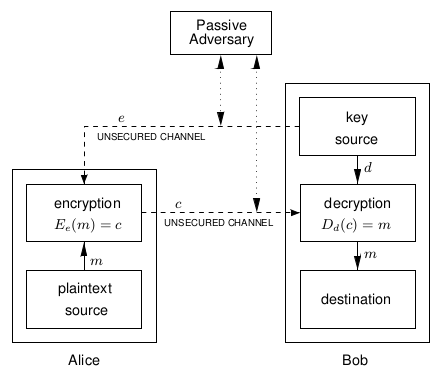
\includegraphics[scale=0.5]{encryption.png}
        \caption{Publikus kulcsú titkosítás \cite{Menezes2001}}
        \label{fig_encryption}
    \end{figure}
\end{frame}

\begin{frame}
    \frametitle{Autentikációs probléma}

    A publikus kulcsú titkosításnál is felvetődik a \textit{man-in-the-middle} probléma.

    \begin{itemize}
        \item Tegyük fel, hogy $A$ üzenetet akar küldeni $B$-nek.
        \item Ahhoz, hogy ezt a publikus kulcsú titkosítás alkalmazásával megtehesse, először meg kell szereznie a
              publikus kulcsot.
        \item A publikus kulcs megszerzése nem biztonságos csatornán keresztül történik (ha biztonságos lenne a csatorna,
              akkor akár szimmetrikus kulcsú titkosítást is használhatnánk).
        \item Tegyük fel, hogy $A$ üzenetet küld, amiben elkéri $B$ publikus kulcsát, viszont $C$ elfogja ezt az üzenetet,
              és elküldi $A$-nak a saját publikus kulcsát.
        \item Ebben az esetben a $B$-nek küldött üzeneteket már $C$ nem csak elfogja, hanem el is tudja olvasni.
    \end{itemize}

    \textbf{Következtetés:} Meg kell bizonyosodni róla, hogy a publikus kulcs, amit $A$ megkap valóban $B$-hez tartozik.
\end{frame}

\begin{frame}
    \frametitle{Digitális aláírás}

    Digitális aláírással hitelesíthetjük a kapott kulcsot. Ez akkor kivitelezhető, ha a titkosítás megfordítható, azaz

    \[D_d(E_e(m)) = E_e(D_d(m)) = m, \forall m \in M \text{ where $M$ is the message space}\]

    Szintén szükséges, hogy az üzenettér és a kódszó tér ugyanaz legyen: $M = C$, ahol $C$ a kódszó tér.
\end{frame}

\begin{frame}
    \frametitle{Digitális aláírás (folytatás)}

    Legyen adott az üzenetszó térnek egy altere ($M'$), aminek mérete lényegesen kisebb, mint $M$ mérete.
\end{frame}

\begin{frame}
    \frametitle{RSA}

    \begin{itemize}
        \item A legismertebb publikus kulcsú titkosítás az RSA algoritmus.
        \item Az algoritmus a kidolgozóiról kapta a nevét: Ron \textbf{R}ivest, Adi \textbf{S}hamir és \textbf{L}eonard Adleman.
        \item 1977-ben publikálták.
        \item Egy ekvivalens verzióját 1973-ban már Clifford Cock már kidolgozta a GCHQ (Government Communication Headquarters),
              amelyet csak 1997-ben hoztak nyilvánosságra.
        \item Előnye, hogy nem kell titkos kulcsot átküldeni annak, akivel kommunikálni szeretnénk.
        \item Hátránya, hogy lényegesen lassabb vele a titkosítás, mint szimmetrikus (egy kulcsú) titkosítási módszerekkel.
        \item Ez az oka annak, hogy egész fájlok titkosítására inkább szimmetrikus titkosítási módszereket használnak, miközben
              a szimmetrikus kulcsot aszimmetrikus módon titkosítják.
    \end{itemize}
\end{frame}

\begin{frame}
    \frametitle{Felhasznált irodalom}

    \printbibliography[heading=bibintoc]
\end{frame}

\begin{frame}
    \Huge
    \textbf{Köszönöm a figyelmet!}
\end{frame}

\end{document}